%!TEX root = /home/renaud/Documents/EPL/tfe/latex/tfe.tex
\section{Application of the method on a simple class of problems}
This section can be considered as a kind of \textit{sanity check} of the method: we define a class of problems for which the box decomposition is intuitively obvious and we check that a community detection algorithm applied on the problem allows to find back that box-decomposition. We call that class of problems the \textit{bi-overturner} problems. The domain that we consider is $\Omega = [-L,\,L]\times[0,\,H]$. Bi-overturner problems basically consist of two \textit{overturner-like} circulations models side-by-side. Let $\Omega^- = [-L,\,0[\times[0,\,H]$ and $\Omega^+ =\; ]0,\,L]\times[0,\,H]$. If $\psi(y,z;y_0,z_0)$ denote the streamfunction defined in \eqref{eq:psi_overturner} with parameters $y_0 \in\; ]0,\,L[$ and $z_0 \in\; ]0,\,H[$, then the streamfunction $\psi_2$ of the bi-overturner problems is defined as
\begin{equation} \label{eq:psi_2box}
	\psi_2(y,z) = \left\{ 
		\begin{array}{lrr}
			\psi(L+y,z;y_0,z_0) & \mbox{if} & (y,z) \in \Omega^-,\\
			0 & \mbox{if} & (y,z) \in \{(0,z)\;|\;z \in [0,\,H]\},\\
			-\psi(y,z;L-y_0,z_0) & \mbox{if} & (y,z) \in \Omega^+,\\
		\end{array}
	\right.
\end{equation}
The streamfunction $\psi_2$ has two extrema of equal strengths: a maximum at $(y_0^-,z_0)$ with $y_0^- \triangleq -L+y_0 = -y_0^-$ and a minimum at $(y_0^+,z_0)$ with $y_0^+ \triangleq L-y_0$. The overturner-like circulation is clockwise in $\Omega^-$ and counterclockwise in $\Omega^+$. The horizontal and vertical velocities $v$ and $w$ are given by
\begin{equation} \label{eq:u-psi_2box}
	v = -\frac{\partial \psi_2}{\partial z}, \quad w = \frac{\partial \psi_2}{\partial y}.
\end{equation}
 Isolines are shown in figures \ref{fig:v2box} and \ref{fig:w2box} respectively. The key feature is that $v(0,z) = 0$, namely the horizontal velocity is zero on the whole segment $y = 0$. Hence, if there is no horizontal diffusion, a passive tracer's particle starting in $\Omega^-$ can never reach $\Omega^+$ and conversely. In that case, we can imagine that there is a vertical wall implying no-through boundary conditions at $y=0$ and the graph is not ergodic. But if the horizontal diffusivity is nonzero in some area near $y=0$, then exchange of particles between $\Omega^-$ and $\Omega^+$ can happen in that area. Now we suppose that the diffusivity tensor $\b K$ is diagonal:
 \begin{equation}
 	\b K(y,z) = \begin{pmatrix} K_h(y,z) & 0\\ 0 & K_v \end{pmatrix}.  	
 \end{equation} 
We assume that the vertical diffusivity $K_v$ is constant and equal to $10^{-3}$ [$\rm{m^2/s}$]. Now we introduce the parameter $\alpha \in [0,1]$ and define $z^* = \alpha H$. We choose an horizontal diffusivity $K_h$ of the form
\begin{equation} \label{eq:Kh2box}
	K_h(y,z) = \begin{cases}
			10^4\ \rm{[m^2/s]} & \mbox{if} \quad y_0^- \le y \le y_0^+ \quad \mbox{and} \quad z^* \le z \le H,\\
			10^3\ \rm{[m^2/s]} & \mbox{if} \quad -L \le y < y_0^- \quad \mbox{or} \quad y_0^+ < y \le L,\\
			0\ \rm{[m^2/s]}  & \mbox{otherwise}.
		\end{cases}
\end{equation}
Now, exchange between $\Omega^-$ and $\Omega^+$ is possible but only above $z^*$.\footnote{From a numerical, random-walk, point of view, we should also ensure that $y_0^+ = |y_0^-|$ is sufficiently large. If not, it would be numerically possible for particles lying below $z^*$ and before $y_0^-$ (resp. after $y_0^+$) to jump from $\Omega^-$ (resp. $\Omega^+$) to $\Omega^+$ (resp. $\Omega^-$).} For the next, we call \textit{exchange zone} the area where $K_v = 10^4$ $\rm{[m^2/s]}$ (dark gray zone in figure \ref{fig:Kh2box}) Hence, we can imagine that there is a vertical, no-through wall of height $z^*$ at $y=0$. The situation is depicted on figure \ref{fig:Kh2box}. Making $\alpha$ vary between $0$ and $1$ defines a class of bi-overturner problem where the vertical wall's height $z^*$ at $y=0$ vary between $0$ and $H$. Two examples of trajectories with the same initial condition are shown for $\alpha = 0.75$ in figures \ref{fig:withouttransfer} and \ref{fig:withtransfer}.

\begin{figure}[!htp]
	\centering
	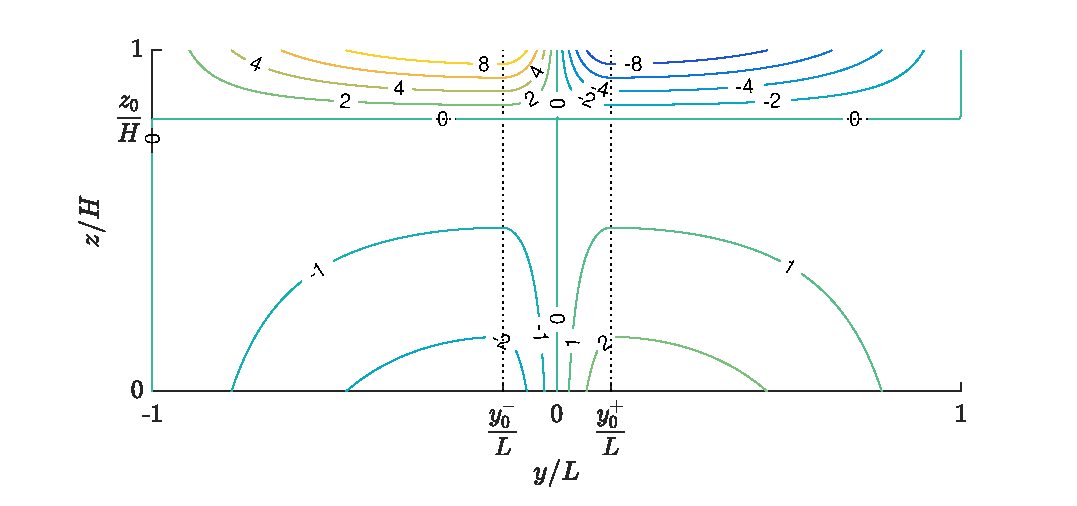
\includegraphics[width=\textwidth]{fig/problem2box/v2box_timmermans.eps}
	\caption{Isolines of the horizontal velocity $v$ for bi-overturner problems.}
	\label{fig:v2box}
\end{figure}

\begin{figure}[!htp]
	\centering
	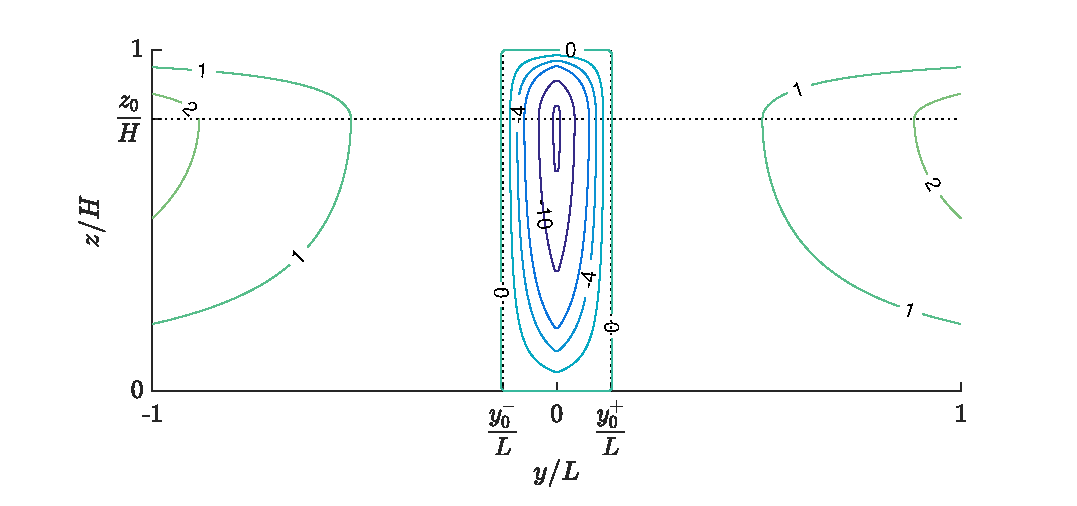
\includegraphics[width=\textwidth]{fig/problem2box/w2box_timmermans.eps}
	\caption{Isolines of the horizontal velocity $w$ for bi-overturner problems.}
	\label{fig:w2box}
\end{figure}

\begin{figure}[!htp]
	\centering
	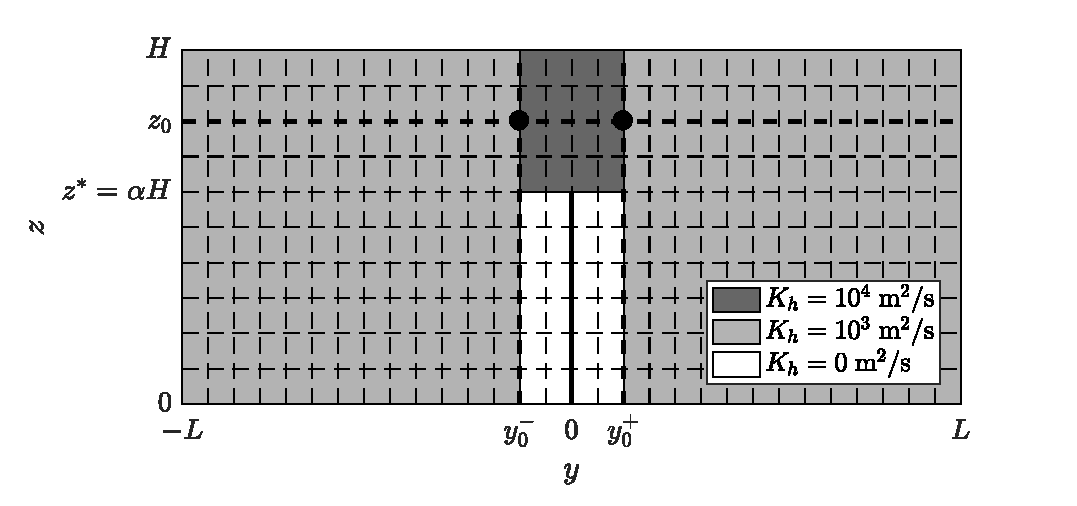
\includegraphics[width=\textwidth]{fig/problem2box/problem.eps}
	\caption{Illustration of the decomposition of the domain into boxes corresponding to the nodes of the directed graph. The values of $K_h$ are also shown for $\alpha = 0.6$, and the fictitious wall is represented by the black continuous line. Here the particle enters the exchange zone but finally stays in $\Omega^-$.}
	\label{fig:Kh2box}
\end{figure}

\begin{figure}[!htp]
	\centering
	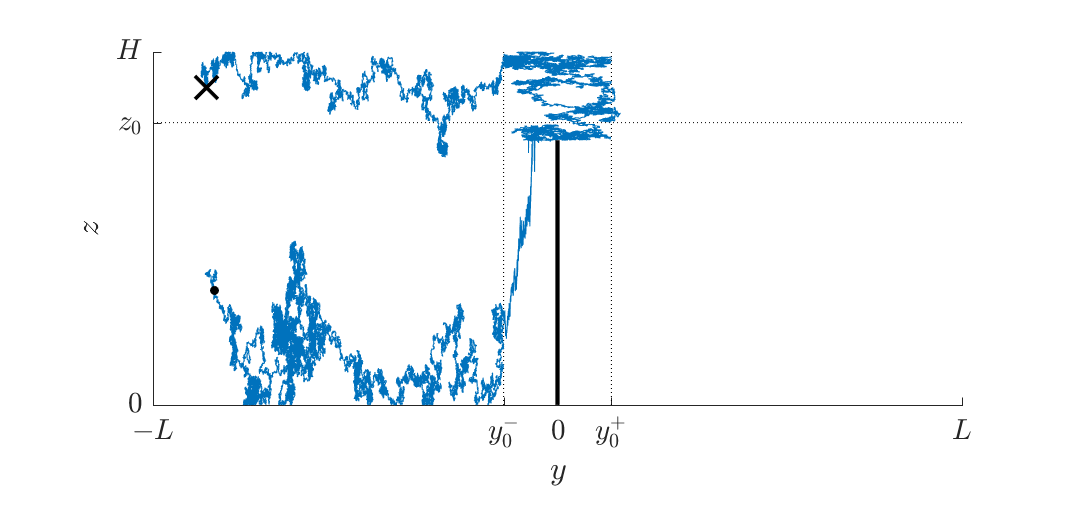
\includegraphics[width=\textwidth]{fig/problem2box/traj_without_transfer5.eps}
	\caption{Example of a particle trajectory in the bi-overturner model with $\alpha = 0.75$. The black cross represents the initial position whereas the black dot shows the final position. The simulation time is 200 years.}
	\label{fig:withouttransfer}
\end{figure}

\begin{figure}[!htp]
	\centering
	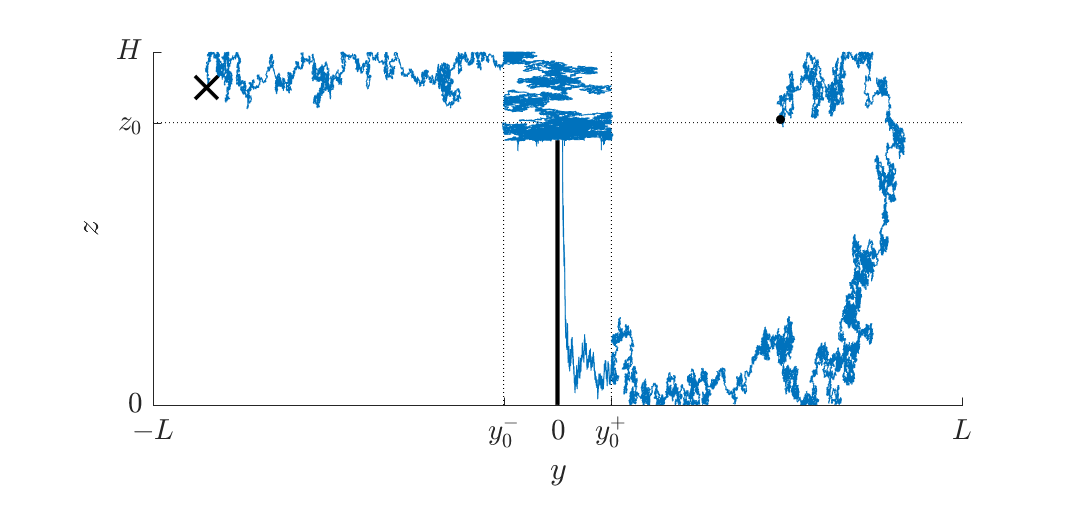
\includegraphics[width=\textwidth]{fig/problem2box/traj_with_transfer2.eps}
	\caption{Example of a particle trajectory in the bi-overturner model with $\alpha = 0.75$. The black cross represents the initial position whereas the black dot shows the final position. The simulation time is 200 years.}
	\label{fig:withtransfer}
\end{figure}
When $\alpha = 1$, the obvious compartmental model is made of the two compartments $\Omega^-$ and $\Omega^+$ which do not communicate with each other. Suppose that different amounts of passive tracer are released into $\Omega^-$ and $\Omega^+$ at a given time; the concentration in each compartment tends to become uniform in time due to diffusion, but the concentration in $\Omega^-$ depends only on the initial quantity of tracer released in $\Omega^-$ and similarly for the concentration in $\Omega^+$. At the contrary, when $\alpha = 0$ the concentration tends to become uniform over the whole domain when time goes to infinity. Hence, we can expect three types of partitioning: a three-communities partitioning with left and right compartments and an exchange zone in between; a two-communities partitioning corresponding to $\Omega^-$ and $\Omega^+$; and finally a trivial partitioning with one single community for very long time scales. For intermediate values of $\alpha$, we expect a behavior similar to the case $\alpha = 1$ when $\alpha$ is close to $1$ and similar to the case $\alpha = 0$ when $\alpha$ goes to $0$. 

\subsection{Results}
The partitioning results are presented here for $\alpha = 1$, $\alpha = 0.75$, $\alpha = 0.5$, $\alpha = 0.25$ and $\alpha = 0$. For every value of $\alpha$, the transition probability matrix is computed at $T = 1$ year on a discretization like the one presented in figure \ref{fig:Kh2box}, namely with $\nby = 30$ and $\nbz = 10$. $10\,000$ particles are initially released in every box. The stability software is run using a vector of Markov times taking values between $10$ and $10^3$. Since we have computed the transition probability matrix for $T = 1$ year, one unit of Markov time correspond here to one year. Notice that in the case where $\alpha = 1$, the graph is not ergodic (it is composed of two ergodic classes) and a random teleportation probability \mtlb{tau} $= 10^{-3}$ is used when running the stability software. When $\alpha < 1$, \mtlb{tau} $=0$ is used.
The stability, number of communities and variation of information curves are shown in figures \ref{fig:staba1}, \ref{fig:staba75}, \ref{fig:staba5}, \ref{fig:staba25} and \ref{fig:staba0} for different values of $\alpha$. Most robust communities correspond to plateaux in the community curve together with a low variation of information. Whatever the value of $\alpha$, the number of communities goes to $2$ after maximum $50$ years, together with a variation of information that is almost zero. In every case, the two-communities partitioning corresponds as expected to $\Omega^-$ and $\Omega^+$. It is shown in figure \ref{fig:cluster_a25_2} for the case $\alpha = 0.25$. In that case, the boundary is perfectly straight which corresponds to the intuition and is conform to the remark made on page \pageref{remark:straightboundaries}. In some other cases, like when $\alpha = 0.5$, the boundary is not exactly a straight line. The situation is depicted in figure \ref{fig:cluster_a5_2}. However, we have to remember that neither the transition probability matrix nor the stability partitioning is solved exactly. Hence, we can consider that the irregularity in the boundary of the communities is due to those numerical artifacts: if a box-model has to be build from the partitioning shown in figure \ref{fig:cluster_a5_2}, the compartments should of course be chosen with a vertical boundary. This illustrates the fact that when using a community-detection algorithm to build compartments for a box-model, the communities should not be blindly interpreted as being the relevant compartments. In particular, if the boundaries of the communities are almost but not exactly vertical and horizontal, one should consider straight boundaries for the compartments. Community detection should thus be considered as a guide towards choosing relevant compartments, rather than as an exact method.

When $\alpha = 0.75$, a small three-communities plateaux starts appearing around 40 years. This plateau grows as $\alpha$ decreases. The corresponding clusterings are shown in figures \ref{fig:cluster_a25_3} and \ref{fig:cluster_a0_3}, where a community corresponding to the exchange zone appears, as expected.

In figure \ref{fig:staba0} corresponding to the case $\alpha = 0$, peaks corresponding to oscillations between two and three communities are observed around 300 and 400 years. As stated in section \ref{sec:stability}, the number of communities should decrease with time, and those oscillations are thus due to the fact that the stability partitioning is only solved approximately. However, this shows that the two- and three-communities clusterings have similar stabilities at those times. Notice that in that case, we expected to find a single-community partitioning for very long Markov times, which does not appear here. Such a clustering would probably appear if we run the stability software for longer Markov times.

Hopefully this introductory example shows how a community-detection algorithm could be use to build compartment models, and provide intuition about why it could work. The communities found depend on the time scale considered but this is not a problem since it could also be the case for the compartments. Notice that we do not to build compartmental models for the bi-overturner class of problems because the compartments are obvious in this case, and it is thus not the goal of this section. In the next section, the method is applied on the overturner problem and we should try to build a compartmental model for that problem. 

\begin{figure}[!htp]
	\centering
	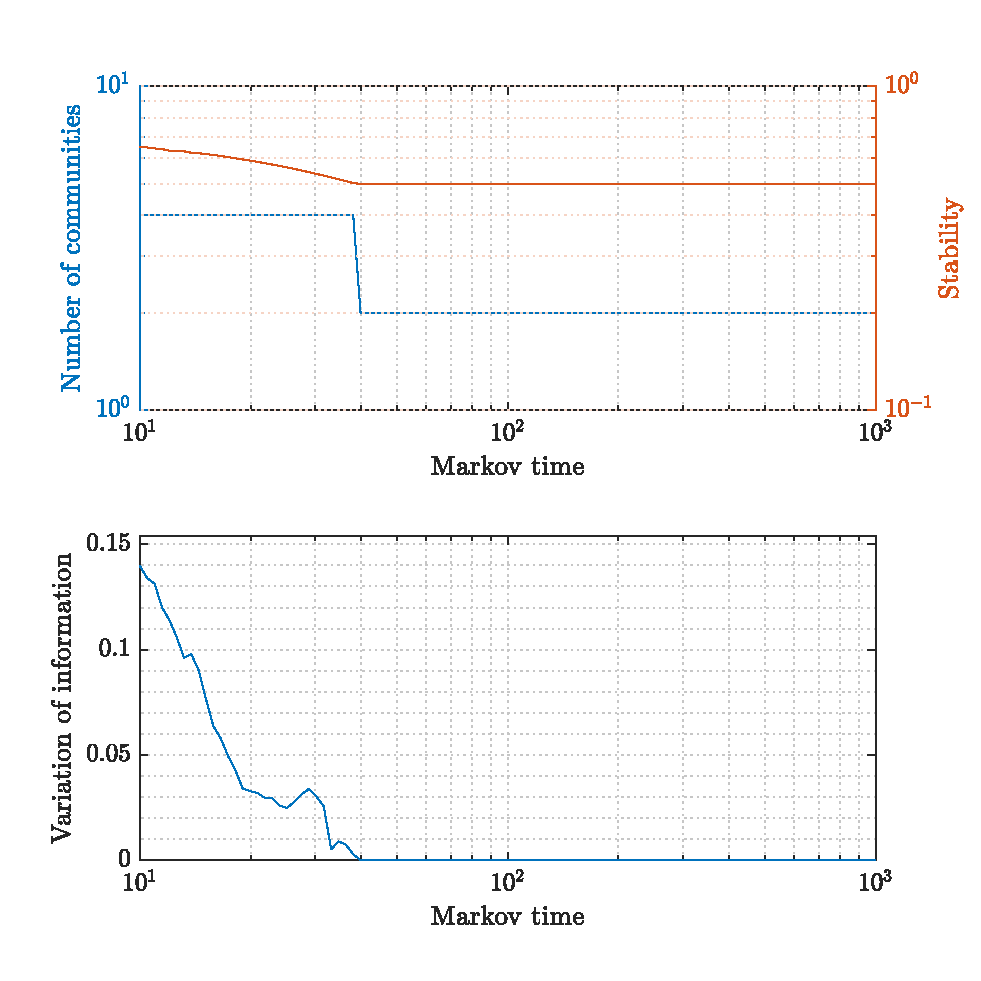
\includegraphics[width = .7\textwidth, height = .4\textheight]{fig/problem2box/stab_a1.eps}
	\caption{Stability, number of communities and variation of information as a function of the Markov time for $\alpha = 1$.}
	\label{fig:staba1}
\end{figure}

\begin{figure}[!htp]
	\centering
	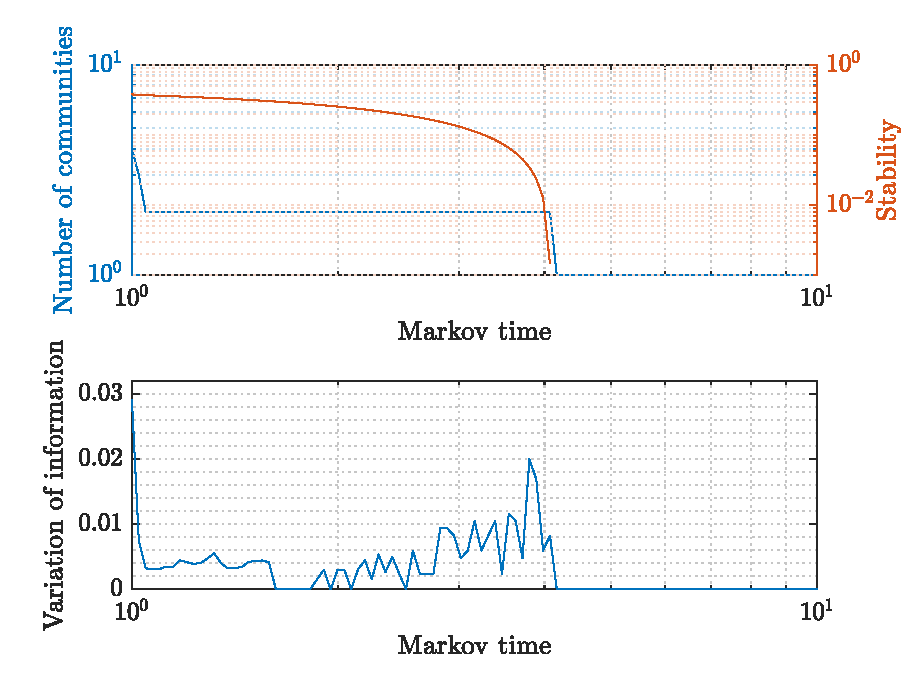
\includegraphics[width = .7\textwidth, height = .4\textheight]{fig/problem2box/stab_a75.eps}
	\caption{Stability, number of communities and variation of information as a function of the Markov time for $\alpha = 0.75$.}
	\label{fig:staba75}
\end{figure}

\begin{figure}[!htp]
	\centering
	\includegraphics[width = .7\textwidth, height = .4\textheight]{fig/problem2box/stab_a5.eps}
	\caption{Stability, number of communities and variation of information as a function of the Markov time for $\alpha = 0.5$.}
	\label{fig:staba5}
\end{figure}

\begin{figure}[!htp]
	\centering
	\includegraphics[width = .7\textwidth, height = .4\textheight]{fig/problem2box/stab_a25.eps}
	\caption{Stability, number of communities and variation of information as a function of the Markov time for $\alpha = 0.25$.}
	\label{fig:staba25}
\end{figure}

\begin{figure}[!htp]
	\centering
	\includegraphics[width = .7\textwidth, height = .4\textheight]{fig/problem2box/stab_a0.eps}
	\caption{Stability, number of communities and variation of information as a function of the Markov time for $\alpha = 0$.}
	\label{fig:staba0}
\end{figure}

\begin{figure}[!htp]
	\centering
	\includegraphics[width = .7\textwidth]{fig/problem2box/cluster_a25_2_.eps}
	\caption{Illustration of the two-communities partitioning for $\alpha = 0.25$.}
	\label{fig:cluster_a25_2}
\end{figure}

\begin{figure}[!htp]
	\centering
	\includegraphics[width = .7\textwidth]{fig/problem2box/cluster_a5_2_.eps}
	\caption{Illustration of the two-communities partitioning for $\alpha = 0.5$.}
	\label{fig:cluster_a5_2}
\end{figure}

\begin{figure}[!htp]
	\centering
	\includegraphics[width = .7\textwidth]{fig/problem2box/cluster_a25_3_.eps}
	\caption{Illustration of the three-communities partitioning for $\alpha = 0.25$.}
	\label{fig:cluster_a25_3}
\end{figure}

\begin{figure}[!htp]
	\centering
	\includegraphics[width = .7\textwidth]{fig/problem2box/cluster_a0_3_.eps}
	\caption{Illustration of the three-communities partitioning for $\alpha = 0$.}
	\label{fig:cluster_a0_3}
\end{figure}